\documentclass{article}

\usepackage[a4paper, top=1in, bottom=1.25in, left=1.25in, right=1.25in]{geometry}
\usepackage{float}

\usepackage{xcolor}
\usepackage[UTF8]{ctex}
\usepackage[colorlinks=true, linkcolor=black, urlcolor=blue]{hyperref}

% For directory structure
\usepackage{dirtree}

% For show image
\usepackage{graphicx}
\usepackage{caption}
\usepackage{subcaption}

\title{Computer Graphics - HW2}
\author{戴旋\ 13331043}

\begin{document}
	\maketitle
	\tableofcontents

	\section{目录结构}

	\dirtree{%
	.1 / \DTcomment{根目录}.
	.2 doc \DTcomment{项目文档}.
	.3 report.tex.
	.3 report.pdf.
	.2 include \DTcomment{FreeGlut 头文件}.
	.2 lib \DTcomment{FreeGlut静态库}.
	.2 obj \DTcomment{存储中间文件}.
    .2 results \DTcomment{实验结果的截图}.
    .3 1.png \DTcomment{第一题}.
    .3 2.png \DTcomment{第二题}.
	.2 src.
	.3 main.cpp \DTcomment{源代码}.
	.2 x64
	.3 freeglut.dll \DTcomment{FreeGlut动态库 x64}.
	.2 freeglut.dll \DTcomment{FreeGlut动态库 x32}.
	.2 main1.exe \DTcomment{第一题的可执行文件}.
	.2 main2.exe \DTcomment{第二题的可执行文件}.
	.2 Makefile \DTcomment{GNU Make}.
	.2 premake5.lua \DTcomment{premake5 脚本}.
	}

	\section{如何运行}
	\textbf{NOTE}:由于有两题,我写在了同一个cpp文件中。Makefile 默认生成的第二题的结果,如果需要生成第一题的结果,请将\textit{glutDisplayFunc}与\textit{glutReshapeFunc}的参数换成\textit{render1}与\textit{reshape1}。
	\begin{enumerate}
		\item Windows 或 Linux:\& GNU Make \& GCC
		\begin{itemize}
			\item Windows可直接运行main1/2.exe (缺少freeglut.dll时,根目录与x64目录下有32位与64位的动态库,可尝试一下)
			\item 在根目录下运行 make 编译生成可执行文件
		\end{itemize}
		\item Mac 或 以上方法无效时,请下载\href{http://premake.github.io/index.html}{premake5},配置好环境变量后,在控制台运行\textbf{premake5 --help}可查看支持的环境。然后在根目录运行\textbf{premake5 xxx}生成相应环境的配置文件。(支持VS,gmake,Xcode)
	\end{enumerate}
	
	\section{程序运行结果}
	\begin{figure}[H]
		\centering
		\begin{subfigure}{0.45\textwidth}
			% pt = px * 72 / DPI
			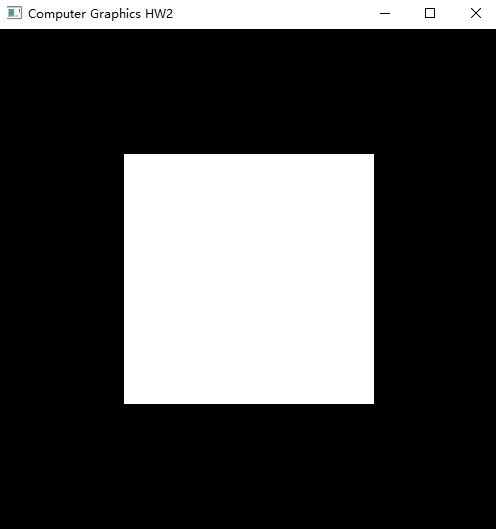
\includegraphics[width=192pt]{../results/1.png}
			\caption{PART-1}
		\end{subfigure}
		~
		\begin{subfigure}{0.45\textwidth}
			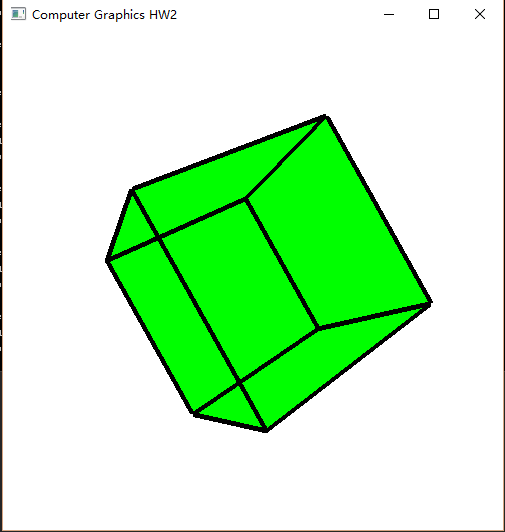
\includegraphics[width=192pt]{../results/2.png}
			\caption{PART-2}
		\end{subfigure}
		\caption{实验结果}
	\end{figure}
\end{document}